\section{Primary clean-source study results}\label{sec:point}
\paragraph{Clean-source release-study results.}
This is a new end-to-end execution of the smaller study, with identical historical periods and model search budget; it is not an exact replication of the full-size historical experiment. The pre-build source tag is \texttt{agdata-research-source-v1}. Both feature tables were rebuilt, with source/input/executable snapshots checked before and after execution. The fixed historical panel is an explicitly hashed external input, not a reproduced panel-selection process. Source attribution is stronger than in the earlier runs, but an observed execution log is not an independent build witness. All results remain retrospective and conditional on the fitted models and observed panel.
Across the eight fits, observed pooled MAE reductions are 4.4--5.9\%, or INR 9.92--18.83 per quintal. Table~\ref{tab:release_point} gives absolute errors and exposure. These gains are descriptive historical differences, not evidence of profitable farmer decisions or independent LightGBM superiority over Spark models. MASE excludes 4.4--4.5\% of rows lacking positive finite training scales, and therefore describes a different population from full-row MAE.

\begin{table*}[!t]\centering\small\setlength{\tabcolsep}{3pt}
\caption{Clean-source release study: candidate/persistence MAE in INR per quintal, forecast rows, calendar days and MASE-excluded rows. Forecast rows are not independent replicates.}\label{tab:release_point}
\begin{tabular}{@{}llrrrrr@{}}\toprule
Regime & Horizon & Rows & Days & MAE C/P & Rel. MAE & MASE omitted\\\midrule
cleaned & next & 553,793 & 294 & 192.34/202.26 & 0.951 & 24,276 \\
cleaned & h3 & 531,316 & 292 & 238.61/252.95 & 0.943 & 24,008 \\
cleaned & h7 & 519,244 & 288 & 301.36/317.31 & 0.950 & 22,739 \\
cleaned & h14 & 496,298 & 281 & 393.48/411.51 & 0.956 & 22,305 \\
unfiltered & next & 554,112 & 294 & 197.04/207.30 & 0.951 & 24,292 \\
unfiltered & h3 & 531,606 & 292 & 243.52/258.90 & 0.941 & 24,024 \\
unfiltered & h7 & 519,527 & 288 & 307.13/323.36 & 0.950 & 22,756 \\
unfiltered & h14 & 496,581 & 281 & 397.39/416.21 & 0.955 & 22,321 \\
\bottomrule\end{tabular}

\end{table*}

\begin{table*}[!t]\centering\small\setlength{\tabcolsep}{3pt}
\caption{Circular-block relative-MAE percentile sensitivity intervals (2,000 replicates, nominal 95\%). Actual coverage is unvalidated; all block specifications are shown.}\label{tab:release_circular}
\begin{tabular}{@{}llrrr@{}}\toprule
Regime & Horizon & 28 days & 42 days & 56 days\\\midrule
cleaned & next & [0.947, 0.955] & [0.947, 0.955] & [0.947, 0.955] \\
cleaned & h3 & [0.940, 0.948] & [0.940, 0.947] & [0.940, 0.947] \\
cleaned & h7 & [0.946, 0.953] & [0.946, 0.953] & [0.946, 0.953] \\
cleaned & h14 & [0.952, 0.961] & [0.953, 0.961] & [0.953, 0.960] \\
unfiltered & next & [0.945, 0.955] & [0.946, 0.955] & [0.946, 0.955] \\
unfiltered & h3 & [0.936, 0.946] & [0.936, 0.945] & [0.936, 0.945] \\
unfiltered & h7 & [0.946, 0.954] & [0.946, 0.954] & [0.946, 0.954] \\
unfiltered & h14 & [0.949, 0.960] & [0.950, 0.959] & [0.952, 0.958] \\
\bottomrule\end{tabular}

\end{table*}

\begin{table*}[!t]\centering\small\setlength{\tabcolsep}{3pt}
\caption{Non-circular-block sensitivity intervals under the same settings. Long blocks leave few temporal spans and do not establish stationarity or future transportability.}\label{tab:release_noncircular}
\begin{tabular}{@{}llrrr@{}}\toprule
Regime & Horizon & 28 days & 42 days & 56 days\\\midrule
cleaned & next & [0.946, 0.955] & [0.946, 0.955] & [0.947, 0.955] \\
cleaned & h3 & [0.939, 0.947] & [0.939, 0.947] & [0.940, 0.947] \\
cleaned & h7 & [0.946, 0.954] & [0.946, 0.953] & [0.946, 0.952] \\
cleaned & h14 & [0.952, 0.962] & [0.952, 0.961] & [0.953, 0.959] \\
unfiltered & next & [0.946, 0.956] & [0.946, 0.955] & [0.947, 0.955] \\
unfiltered & h3 & [0.938, 0.946] & [0.939, 0.946] & [0.939, 0.946] \\
unfiltered & h7 & [0.946, 0.955] & [0.947, 0.955] & [0.947, 0.954] \\
unfiltered & h14 & [0.951, 0.961] & [0.952, 0.960] & [0.953, 0.958] \\
\bottomrule\end{tabular}

\end{table*}
The sensitivity interval endpoints across all six specifications and eight fits span 0.936--0.962; this range is not a combined confidence interval. State and commodity summaries contain 46 group-by-fit comparisons with relative MAE above one; all subgroup counts and errors are retained, without selecting favourable subgroups. Groups and fits overlap, so this count is descriptive, not a multiplicity-adjusted finding.

The daily diagnostics in Figure~\ref{fig:release_dependence} display loss differences, exposure and autocorrelation for the cleaned 7-day fit; diagnostics for all fits are recorded with the release. Substantial long-range correlation, seasonal changes or exposure variation can invalidate short-memory approximations. HAC bandwidth sensitivity is secondary: no horizon correction is claimed and tiny p values are not evidence of validated inference. Independent entity-resampling intervals are exploratory and cannot establish generalisation to independent new markets. Human expert statistical review and genuinely future-issued evaluation remain outstanding.
\begin{figure}[!t]\centering
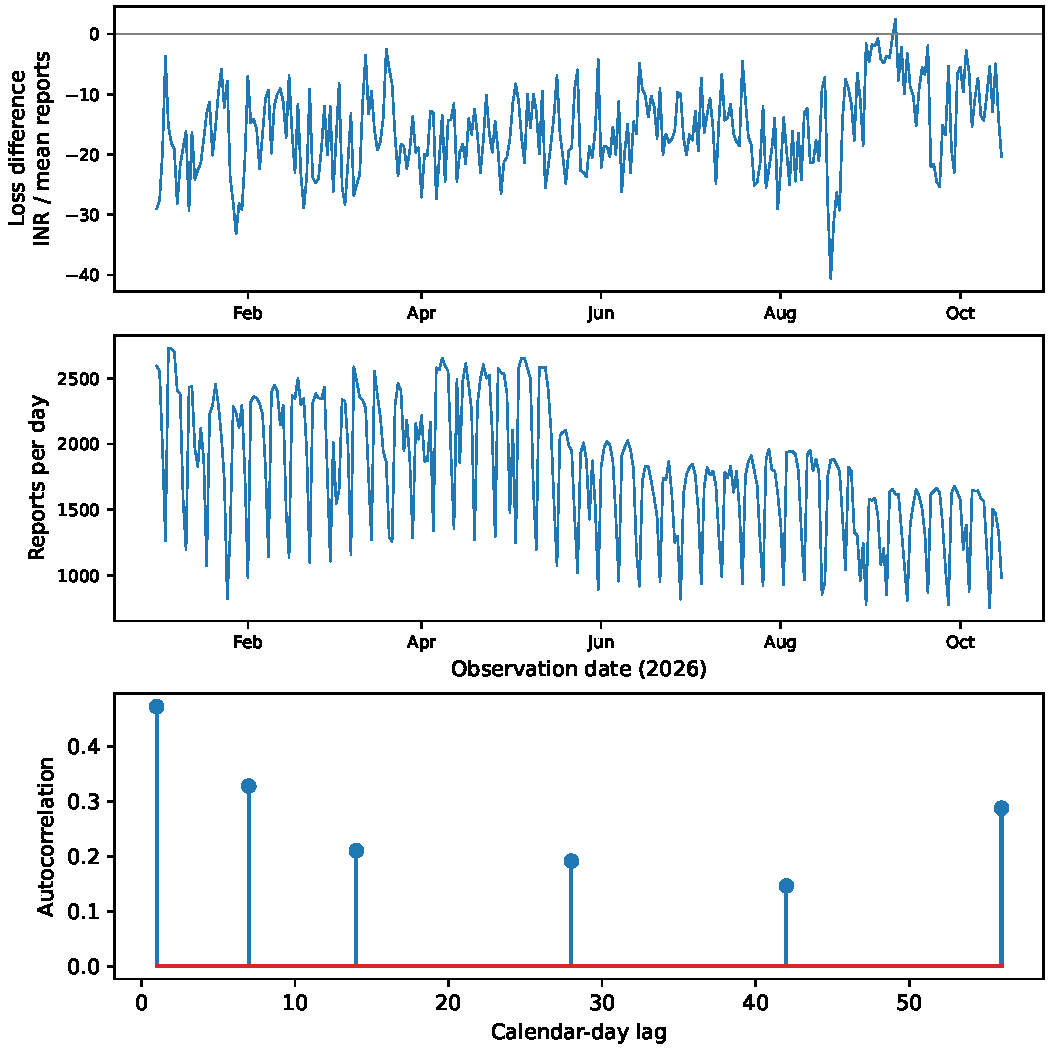
\includegraphics[width=0.88\linewidth]{release_dependence.pdf}
\caption{Release cleaned 7-day daily candidate-minus-persistence total loss divided by mean daily exposure (top), report counts (middle), and descriptive autocorrelation (bottom). No independence threshold is asserted.}\label{fig:release_dependence}
\end{figure}

